%----------------------------------------------------------------------------------------
%
% LaTeX-template for degree projects at LNU, Department of Computer Science
% Last updated by Johan Hagelbäck, Oct 2015
% Linnaeus University
%
% License: Creative Commons BY
%
%----------------------------------------------------------------------------------------

%----------------------------------------------------------------------------------------
%	Settings and configuration
%----------------------------------------------------------------------------------------

\documentclass[a4paper,12pt]{article}
\usepackage[T1]{fontenc}
\usepackage{times}
\usepackage[english]{babel}
\usepackage[utf8]{inputenc}
\usepackage{caption}
\usepackage{subcaption}
\usepackage{wallpaper}
\usepackage[absolute]{textpos}
\usepackage[top=2cm, bottom=2.5cm, left=3cm, right=3cm]{geometry}
\usepackage{appendix}
\usepackage[nottoc]{tocbibind}
\usepackage[hidelinks]{hyperref}
\setcounter{figure}{0}
%\setcounter{secnumdepth}{3}
%\setcounter{tocdepth}{3}
\usepackage{amsmath}
\numberwithin{figure}{section}
\usepackage{sectsty}
\sectionfont{\fontsize{14}{15}\selectfont}
\subsectionfont{\fontsize{12}{15}\selectfont}
\subsubsectionfont{\fontsize{12}{15}\selectfont}

\usepackage{csquotes} % Used to handle citations

\renewcommand{\thetable}{\arabic{section}.\arabic{table}}  
\renewcommand{\thefigure}{\arabic{section}.\arabic{figure}} 

%----------------------------------------------------------------------------------------
%	
%----------------------------------------------------------------------------------------
\newsavebox{\mybox}
\newlength{\mydepth}
\newlength{\myheight}

\newenvironment{sidebar}%
{\begin{lrbox}{\mybox}\begin{minipage}{\textwidth}}%
{\end{minipage}\end{lrbox}%
 \settodepth{\mydepth}{\usebox{\mybox}}%
 \settoheight{\myheight}{\usebox{\mybox}}%
 \addtolength{\myheight}{\mydepth}%
 \noindent\makebox[0pt]{\hspace{-20pt}\rule[-\mydepth]{1pt}{\myheight}}%
 \usebox{\mybox}}

%----------------------------------------------------------------------------------------
%	Title section
%----------------------------------------------------------------------------------------
\newcommand\BackgroundPic{
    \put(-2,-3){
    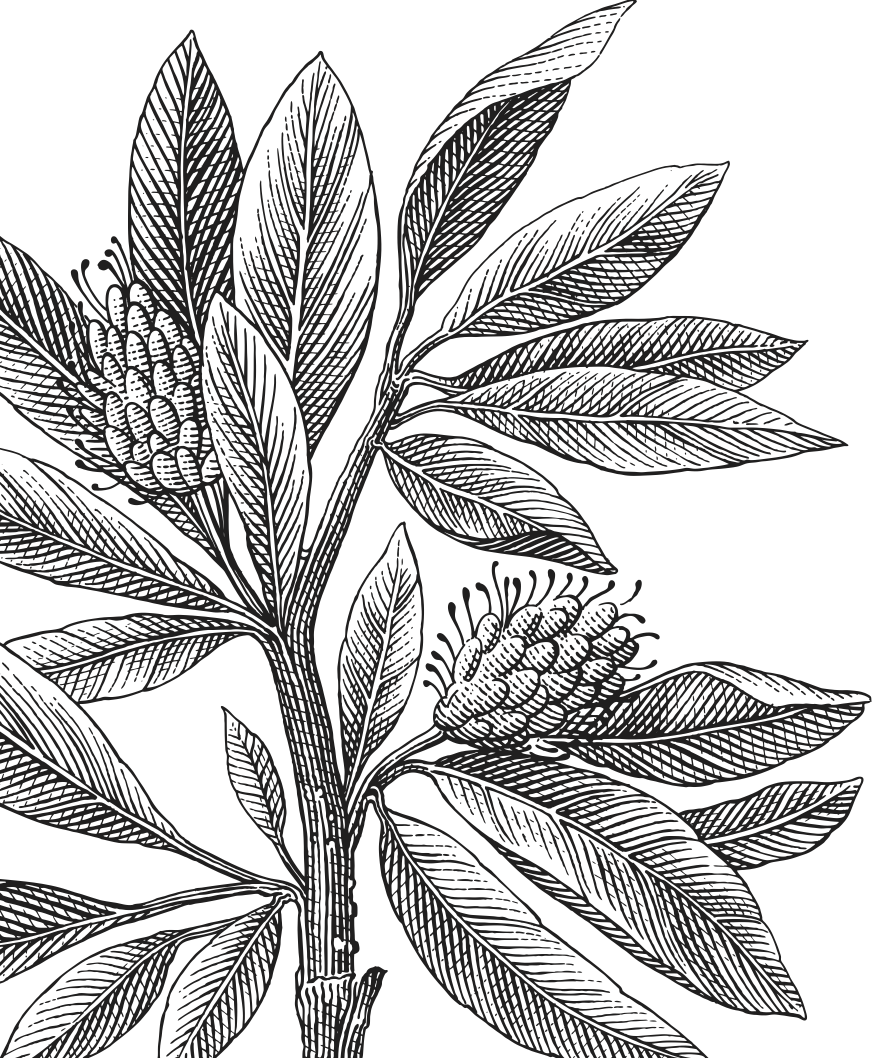
\includegraphics[keepaspectratio,scale=0.3]{img/lnu_etch.png} % Background picture
    }
}
\newcommand\BackgroundPicLogo{
    \put(30,740){
    
\includegraphics[keepaspectratio,scale=0.10]{img/logo.png} % Logo in upper left corner
    }
}

\title{	
\vspace{-8cm}
\begin{sidebar}
    \vspace{10cm}
    \normalfont \normalsize
    %\Huge Bachelor/Master Thesis Project \\
    \vspace{-1.3cm}
\end{sidebar}
\vspace{3cm}
\begin{flushleft}
    \huge Computer networks - 1DV701 \\ 
    \LARGE  Assignment 3\\
\end{flushleft}
\null
\vfill
\begin{textblock}{6}(10,13)
\begin{flushright}
\begin{minipage}{\textwidth}
\begin{flushleft} \large
\emph{Author:} Michael Johansson \& Jakob Heyder\\ % Author
%\emph{Supervisor:} Name of your supervisor\\ % Supervisor
%\emph{Examiner:} Dr.~Mark \textsc{Brown}\\ % Examiner (course manager)
\emph{Semester:} VT 2017\\ % 
%\emph{Subject:} Computer Science\\ % Subject area
\end{flushleft}
\end{minipage}
\end{flushright}
\end{textblock}
}

\date{} 

\begin{document}
\pagenumbering{gobble}
\newgeometry{left=5cm}
\maketitle
\clearpage


%----------------------------------------------------------------------------------------
\newpage
\pagenumbering{gobble}
\tableofcontents % Table of contents
\newpage
\pagenumbering{arabic}

%----------------------------------------------------------------------------------------
%
%	Here follows the actual text contents of the report.
%
%----------------------------------------------------------------------------------------

\section{Assignment summary}

\begin{itemize}
\item\textbf{Michael}
Work percentage 50\%

\item\textbf{Jakob} 
Work percentage 50\%
\end{itemize}



\newpage

\section{Problem one}

In figure \ref{TFTP_READ} we show a successful RRQ (Read-Request) to the implemented tftp server retrieving a small test-text file.
\noindent
We use the original socket as a kind of server socket accepting the requests on port 4970 (Usually 69 in FTP) and then after receiving a request, either write or read, we open a new thread for the specific client connection. In this thread we use the sending socket which acquires a free port (zero port indicates to get a random free port e.g. 5800) and then send the new specified port to the client in the ACK (WRQ) or DATA (RRQ) packet.  This is defined in the TFTP-Specification that the initialization will be on a predefined port and then the server communicates the used port to the client. This way we can also handle multiple client requests since the original socket is freed after handling the client in a separate thread. Also the send socket connects to the remote port and address of the client given from the request.

\begin{figure}[h!]
	\centering
	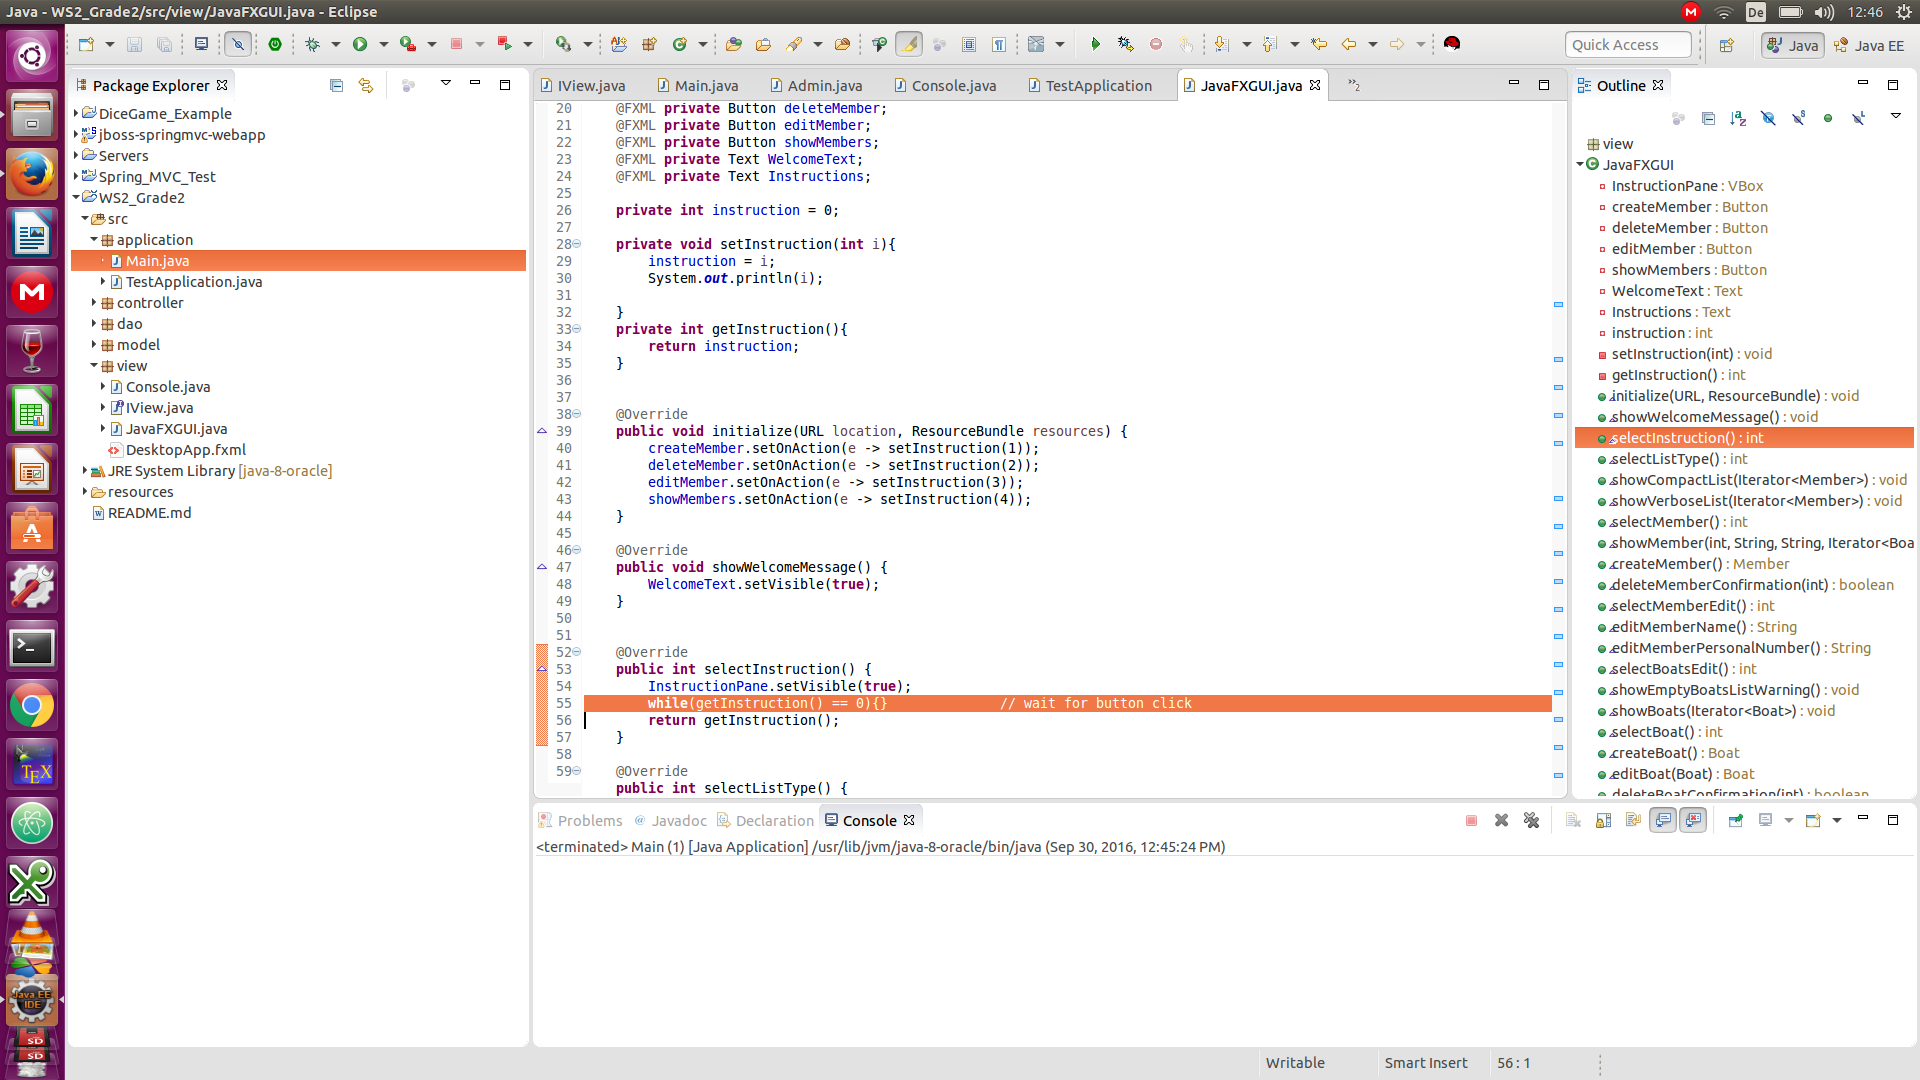
\includegraphics[width=0.95\textwidth,keepaspectratio]{img/problem1.png} 
	\caption{Successful READ-Request. We can see the tftp-client in the terminal window, eclipse tftp server and the home directory where the retrieved file is saved to.}
	\label{TFTP_READ}
\end{figure}

 

\newpage
\section{Problem two}

In figure \ref{TFTP_READ_WRITE} we send and receive multiple large files. The task says sending but it is not clear if it means sends from client or server. However both is on the screenshot with files larger then 512 bytes. The case of files which are so large that they exceed the package number of a short is thought of but not mentioned in the specification. Therefore its left out and assumed out of scope in this assignment. 

We implemented a timeout mechanism that the sending socket times out if it does not receive the next DATA/ACK packet in 150ms. If it times out it will try to retransmit or simply tries to receive again. We have a retransmission counter which will be increased and stops the execution after 5 retransmissions/waiting-times so that no infinite loop will occur. 

The execution of a write-request can be seen also on figure \ref{TFTP_READ_WRITE}. 

\begin{figure}[h!]
	\centering
	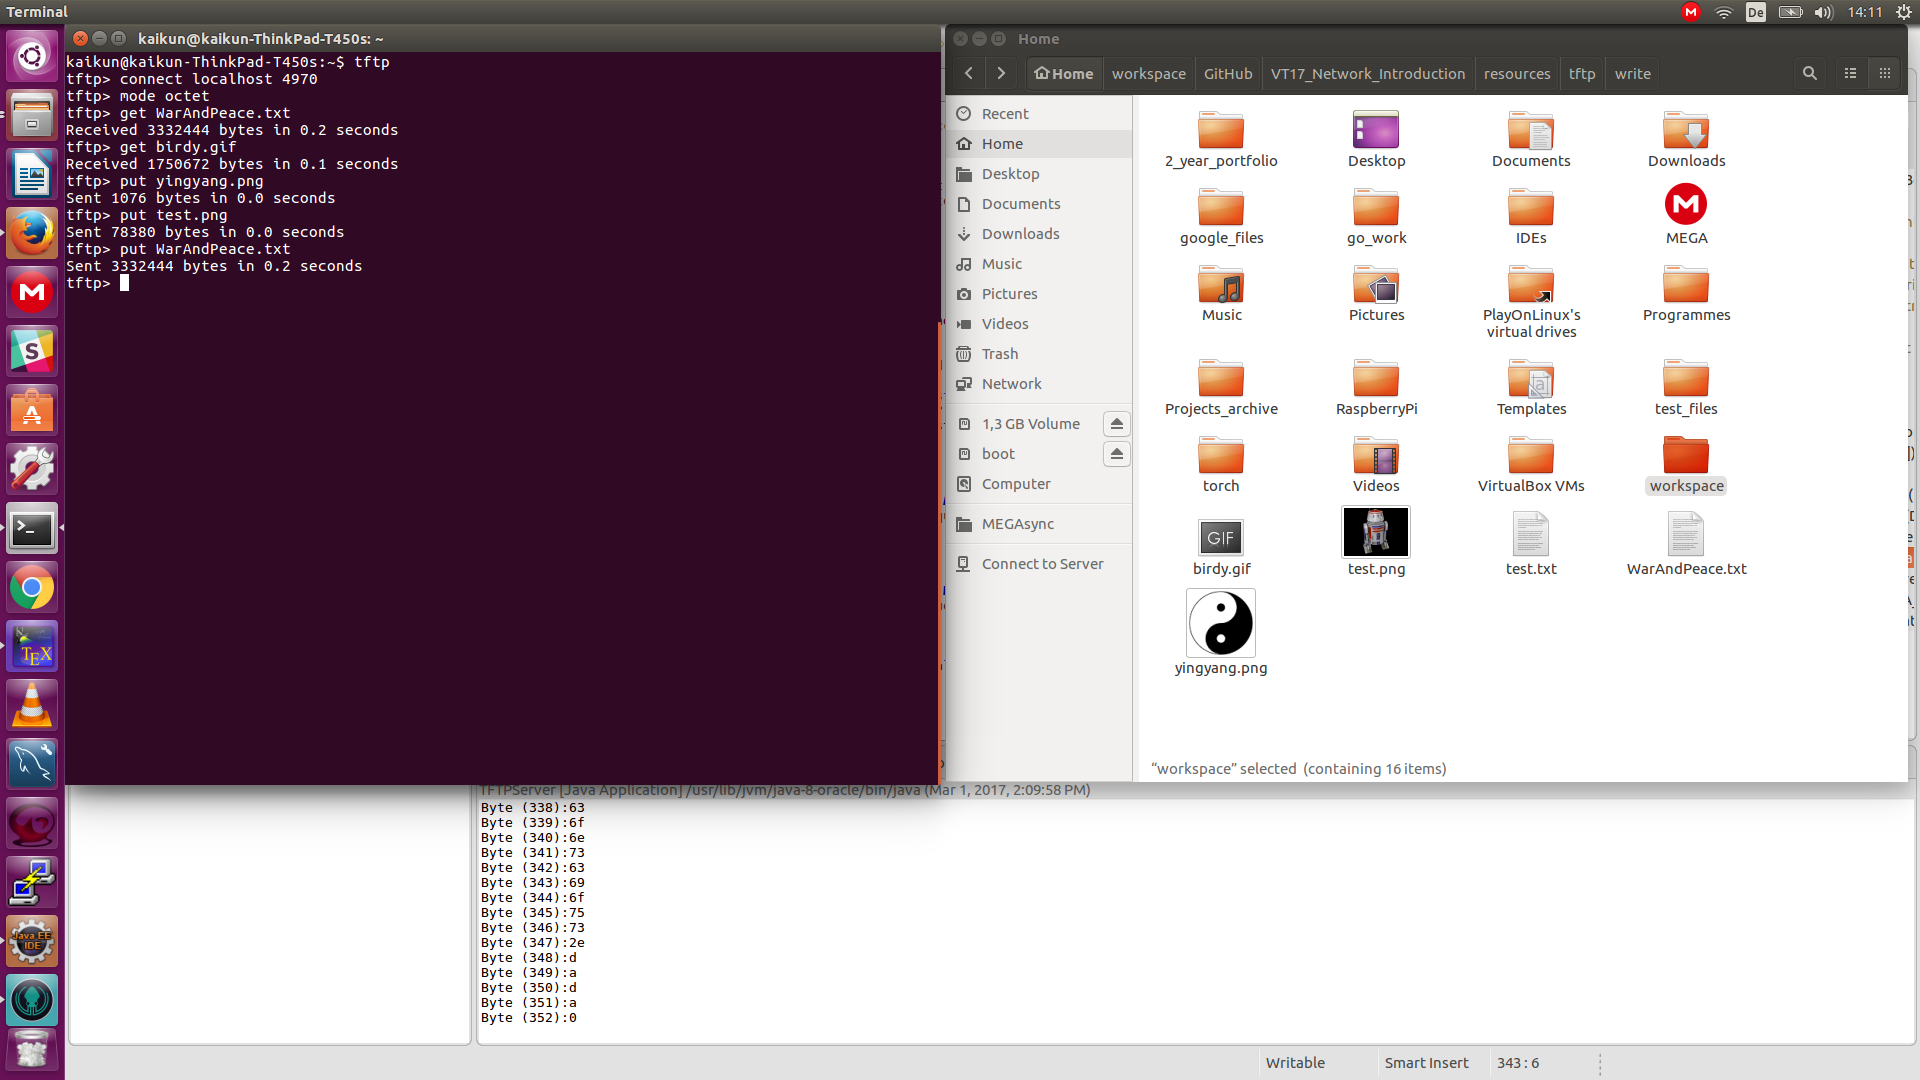
\includegraphics[width=0.95\textwidth,keepaspectratio]{img/ReadWriteMultipleFiles.png} 
	\caption{Read and write multiple large files. On the left hand side we see the tftp client transfering files from the home directory or reading files from the server. We can see the bytes transfered.}
	\label{TFTP_READ_WRITE}
\end{figure}




List of all implemented server responses
\begin{itemize}
	\item 200: OK
	\item 201: Created
	\item 204: No Content
	\item 302: Found
	\item 400: Bad request
	\item 403: Access Denied
	\item 404: Not Found
	\item 411: Length Required
	\item 414: URI Too Long
	\item 415: Unsupported Media Type
	\item 500: Internal Server Error
	\item 501: Not implemented
	\item 505: HTTP Version Not Supported
\end{itemize}


\newpage
\subsection{VG.1 HTTP status code implementation}

For some images below we just show the error.html response but we send the status code as well for every error.



\newpage
\subsection{VG.2 POST vs PUT}

We use POST when the user uploads a new resource that our sever handles where it should be placed. In our POST implementation the user can upload an image through our upload page. The server then creates that images with a hash as the file name and under the images folder.  

If instead the user has the exact request-URI then we can use PUT to create or overwrite the file on that exact URI. 

So in short the POST is used for when the client don't need to know the exact URI and just upload the file where we want it. The PUT when the client want to Create or replace a file on an exact URI.

\newpage

\section{Problem three}


\end{document}
